\newpage
\section{Ho-Kalman辨识算法\label{sec:Ho-Kalman辨识过程介绍}}
\subsection{激励信号的选取}
理论上来说，Ho-Kalman算法对于输入信号没有要求。但是输入信号需要激励出被控系统的主要模态，这要求输入信号频谱尽可能宽，在系统的
主要模态附近的激励能力要远远超出采样噪声。

一种常见的输入激励信号为\textbf{伪随机二进制序列（Pseudo-Random Binary Sequence，PRBS）}中的最大长度序列，记为\textbf{M序列}。
在时域上，M序列表现为以幅值\(\pm A\)不断变换的、间隔为\(T_s\)的、周期为\(2^{N}-1\)的序列。这里点明了M序列的三个核心参数：
幅值\(A\)、采样周期\(T_s\)、级数\(N\)。

M序列的特点是近似为白噪声，自相关尖锐，便于进行相关分析辨识。当然也有坏处。根据功率谱分析可知，M序列在直流分量（0Hz）附近
基本没有激励能力，即采样M序列对于系统的开环放大系数辨识效果很差。因此一般会使用阶跃信号产生直流分量，确定开环放大系数和工作点；然后
在等到系统阶跃响应基本结束后叠加M序列，进行工作点附近的系统辨识。

M序列的三个参数需要慎重选取，这决定着辨识结果：

\begin{itemize}
    \item 幅值\(A\)：一般而言，幅值越高，激励能力越强，信噪比越高。但过高的幅值可能会导致系统偏离工作点附近的线性区间，反而降低
    辨识结果。
    \item 采样周期\(T_s\)：采样周期越高，采样频率越高，辨识结果越好。但采样频率越高，数据采集和上传难度越高。一般选择采样周期
    \(\cfrac{1}{T_s}\ge 10f_c\)，其中\(f_c\)为预估的系统截止频率。
    \item 级数\(N\)：级数越高，伪随机在频域上的频点间隔越小，但相应的每个频点上的激励能力下降。而级数N也影响着辨识时长。对于大部分
    机电系统，推荐选取N=9\(\sim\)12。
\end{itemize}

M序列的产生一般采用反馈移位寄存器实现，代码实现较为简单，只是需要占据很长的一段空间存储。如下是一个给定级数N=11的M序列实现函数，此时周期为\(2^{N}-1=2047\)。输出结果存储在数组m\(\_\)seq[2047]中，用0和1表示结果。

\begin{lstlisting}
void generate_m_sequence_11(unsigned char m_seq[])
{
        uint16_t lfsr = 0x7FF;        // 11位寄存器初始状态（全1）
        const uint16_t mask = 0x7FF;  // 低11位掩码

        for (int i = 0; i < 2047; i++) {
            // 当前输出为寄存器最高位（bit10）
            m_seq[i] = (lfsr >> 10) & 1u;

            // 反馈：bit10 异或 bit1（对应本原多项式 x^11 + x^2 + 1）
            uint16_t feedback = ((lfsr >> 10) ^ (lfsr >> 1)) & 1u;

            // 移位并插入反馈，保持11位有效
            lfsr = ((lfsr << 1) | feedback) & mask;
        }
}
\end{lstlisting}
\subsection{系统脉冲响应的求解}

通过输入伪随机信号，得到了输入序列\(x_k\)和输出序列\(y_k\)，长度为\(M=2^N-1\)。
第一步是计算脉冲响应序列。若离散系统的脉冲响应序列为\(g_k\)，则会满足：
\begin{equation}
    y_k=x_k * g_k
    \label{eq:离散时域卷积方程}
\end{equation}

但是由于采样噪声存在，直接求解上述的离散卷积方程结果往往会很差，因此需要稍作变换（具体原理见
\ref{sec:噪声作用下的相关分析法简介}）。此处需要的不是采样噪声，而是其中的有效信息，
因此可以求解输入信号的\textbf{自相关序列（Self-Correlation Sequence）}：
\footnote{若有时域信号\(x\)和\(y\)，相关运算指的是进行\(R_{xy}(\tau)=\text{E}[x(t)y(t+\tau)]\)，
即在不同的偏移情况下求解两个信号对应元素相乘的期望。若两个信号完全一致（与自身做相关运算）则称为自相关，若不一致则称为互相关。
相关函数特点是，在一定偏移下两个信号的统计学相关性越高，相关函数在此处的值相较于其他地方会更高。若两个信号在没有统计学相关性则相关函数为
\(R_{xy}(\tau)=\text{E}[x(t)]\cdot \text{E}[y(t+\tau)]\)为两者均值之积。
}
\begin{equation*}
    R_{xx}(k)=\cfrac 1M\sum_{i=0}^{M-1} x_{i} x_{i+k} =\cfrac 1M(x_{-k} * x_{k})
\end{equation*}

输入与输出信号的\textbf{互相关序列（Cross-Correlation Sequence）}：
\begin{equation*}
    R_{xy}(k)=\cfrac 1M\sum_{i=0}^{M-1} x_{i} y_{i+k} =\cfrac 1M(x_{-k} * y_{k})
\end{equation*}

其中\(x_{-k}\)表示输入序列\(x_{k}\)的时间反转。
\footnote{相关运算和卷积是类似的，卷积是“信号反转后滑动平均”的过程，而相关运算将一个输入信号反转后卷积，相当于
“信号不反转直接滑动平均”的过程。}
而对于时域卷积方程\ref{eq:离散时域卷积方程}，两边同时与\(x_{-k}\)卷积并乘上序列长度倒数
\(\cfrac 1M\)可得：
\begin{equation*}
    \cfrac 1M x_{-k}*y_k=\cfrac 1Mx_{-k}*x_k*g_k
\end{equation*}

也就可以表示为：
\begin{equation}
    R_{xy}(k)=R_{xx}(k)*g_k
    \label{eq:维纳-霍普夫方程}
\end{equation}

该方程称为\textbf{维纳-霍普夫方程（Wiener-Hopf Equation）}，是相关分析法的核心所在。
该方程表明，通过相关序列变换，可以视为输入了时域自相关序列，输出信号为时域互相关序列。

在得到了输入自相关序列和互相关序列后，接下来需要求解系统的脉冲响应序列，也就是求解维纳-霍普夫方程\ref{eq:维纳-霍普夫方程}。该方程
可以展开为：
\begin{equation*}
    R_{xy}(k)=\sum_{j=0}^{N-1}R_{xx}(k-j)\times g_j
\end{equation*}

可以将其改写为矩阵形式：
\begin{equation*}
    \begin{bmatrix}
        R_{xy}(0)\\
        R_{xy}(1)\\
        \vdots\\
        R_{xy}(N-1)
    \end{bmatrix}
    =
    \begin{bmatrix}
        R_{xx}(0)&R_{xx}(1)&R_{xx}(2)&\cdots&R_{xx}(N-1)\\
        R_{xx}(1)&R_{xx}(0)&R_{xx}(1)&\cdots&R_{xx}(N-2)\\
        R_{xx}(2)&R_{xx}(1)&R_{xx}(0)&\cdots&R_{xx}(N-3)\\
        \vdots&\vdots&\vdots&\ddots&\vdots\\
        R_{xx}(N-1)&R_{xx}(N-2)&R_{xx}(N-3)&\cdots&R_{xx}(0)
    \end{bmatrix}
    \begin{bmatrix}
        g_0\\
        g_1\\
        \vdots\\
        g_{N-1}
       \end{bmatrix}
\end{equation*}

定义向量
\(\textbf{r}_{xy}=\begin{bmatrix}
        R_{xy}(0)\\
        R_{xy}(1)\\
        \vdots\\
        R_{xy}(N-1)
    \end{bmatrix}\)
和\(\textbf{g}=\begin{bmatrix}
        g_0\\
        g_1\\
        \vdots\\
        g_{N-1}
    \end{bmatrix}\)

可以发现矩阵
\(\textbf{r}_{xx}=
    \begin{bmatrix}
        R_{xx}(0)&R_{xx}(1)&R_{xx}(2)&\cdots&R_{xx}(N-1)\\
        R_{xx}(1)&R_{xx}(0)&R_{xx}(1)&\cdots&R_{xx}(N-2)\\
        R_{xx}(2)&R_{xx}(1)&R_{xx}(0)&\cdots&R_{xx}(N-3)\\
        \vdots&\vdots&\vdots&\ddots&\vdots\\
        R_{xx}(N-1)&R_{xx}(N-2)&R_{xx}(N-3)&\cdots&R_{xx}(0)
    \end{bmatrix}
    \)
从左上到右下，每一个对称对角线上的元素均相等（如第一个为\(R_{xx}(0)\)，第二个为\(R_{xx}(1)\)，第三个为\(R_{xx}(2)\)），为
托普利茨矩阵。

通过构造自相关的托普利茨矩阵，可以将离散的卷积方程，改写为矩阵乘法方程：

\begin{equation*}
    \textbf{r}_{xy}=\textbf{r}_{xx}\textbf{g}
\end{equation*}

脉冲响应序列可以通过矩阵求逆计算得到：

\begin{equation}
    \textbf{g}=\textbf{r}_{xx}^{-1}\textbf{r}_{xy}
    \label{eq:脉冲响应序列求解}
\end{equation}

如下图是针对三轴云台方位轴速度环辨识过程中得到的输入相关序列、输入输出自相关序列和脉冲响应序列：

\begin{figure}[H]
    \begin{minipage}{0.5\textwidth}
        \centering
        
\includegraphics[width=0.8\textwidth]
        {图片/输入自相关序列.jpg}
        \caption{输入自相关序列}
        \label{fig:输入自相关序列}
    \end{minipage}
    \begin{minipage}{0.5\textwidth}
        \centering
        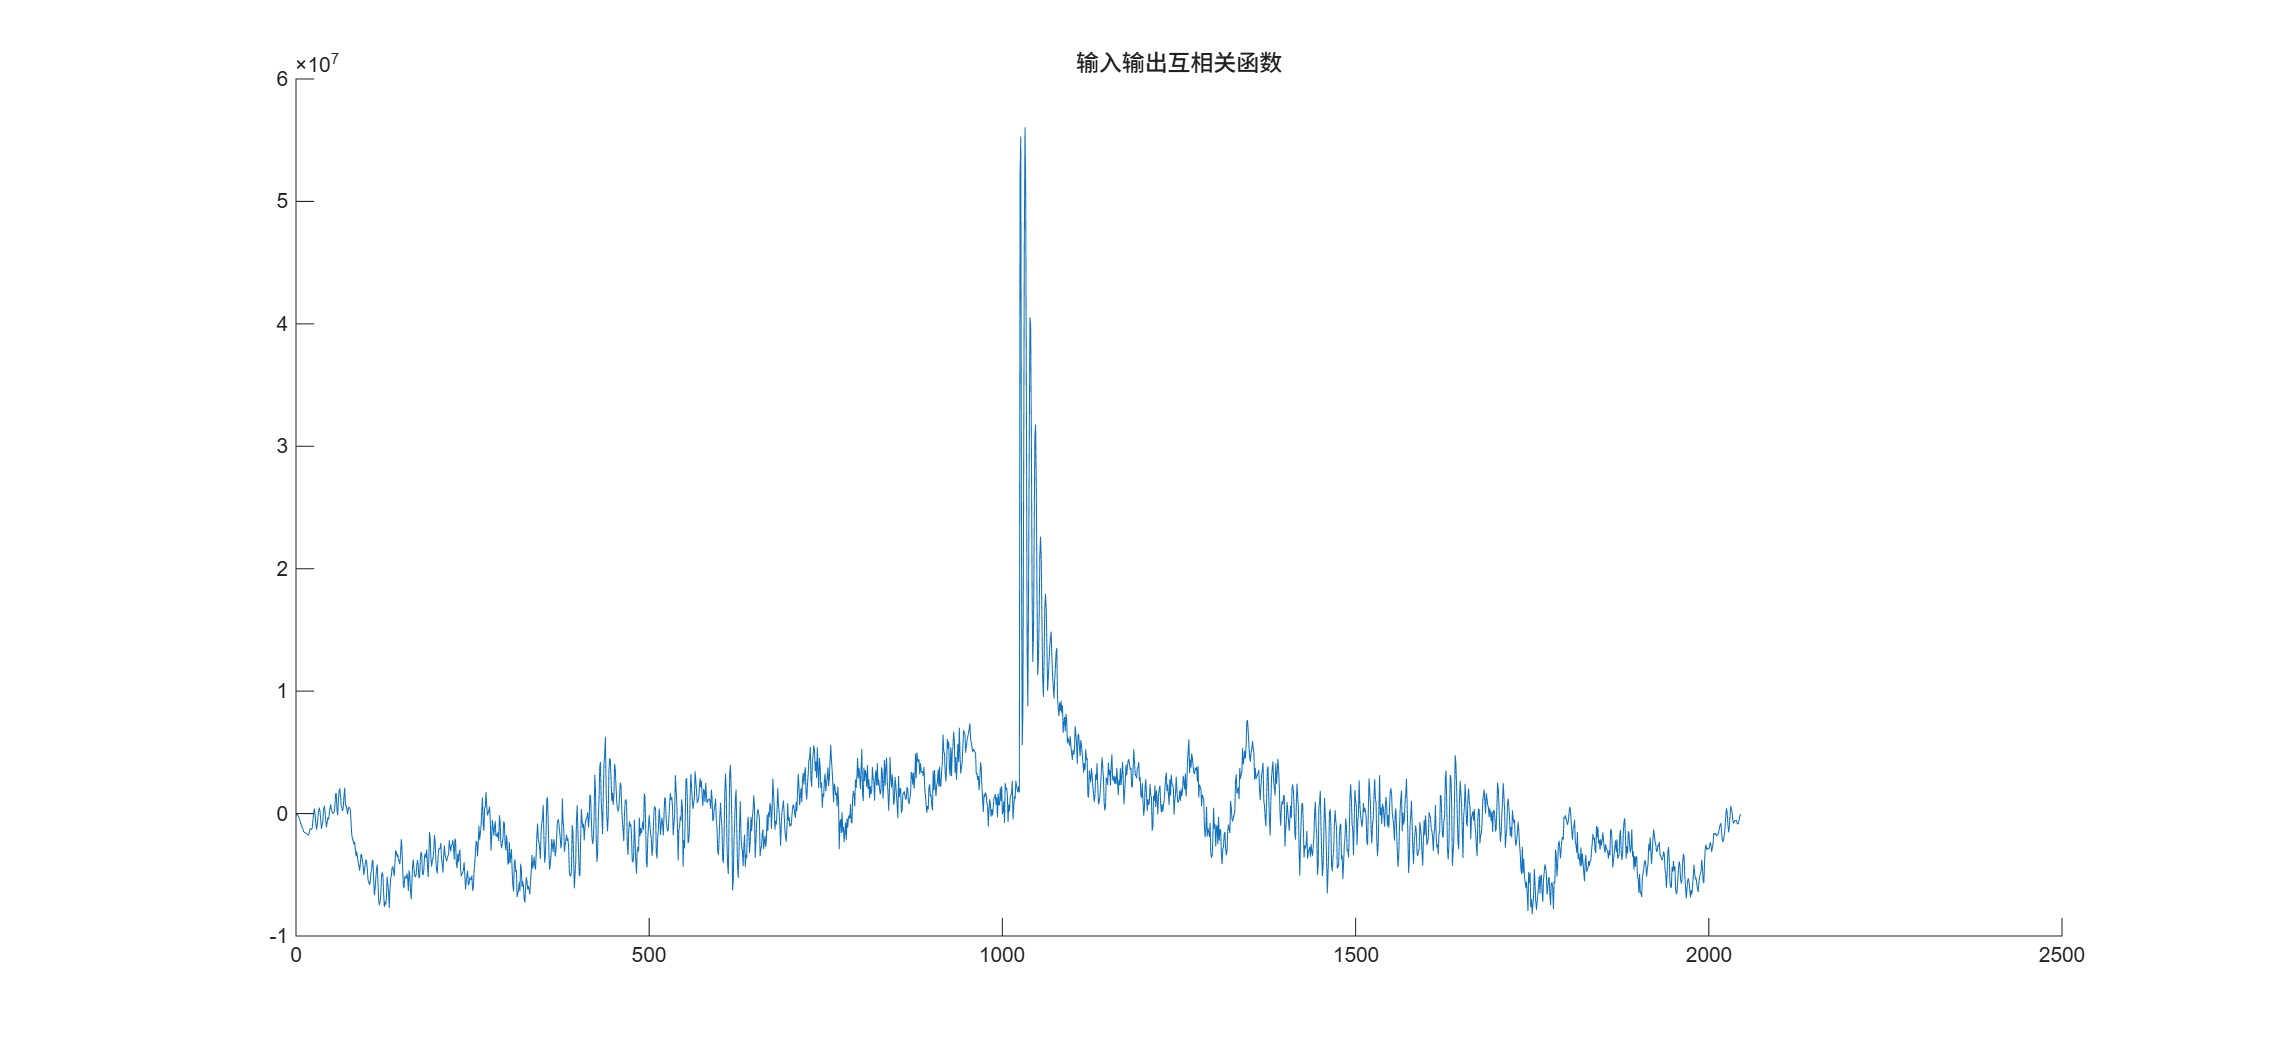
\includegraphics[width=0.8\textwidth]
        {图片/输入输出互相关序列.jpg}
        \caption{输入输出互相关序列}
        \label{fig:输入输出互相关序列}
    \end{minipage}
\end{figure}

\begin{figure}[H]
    \centering
    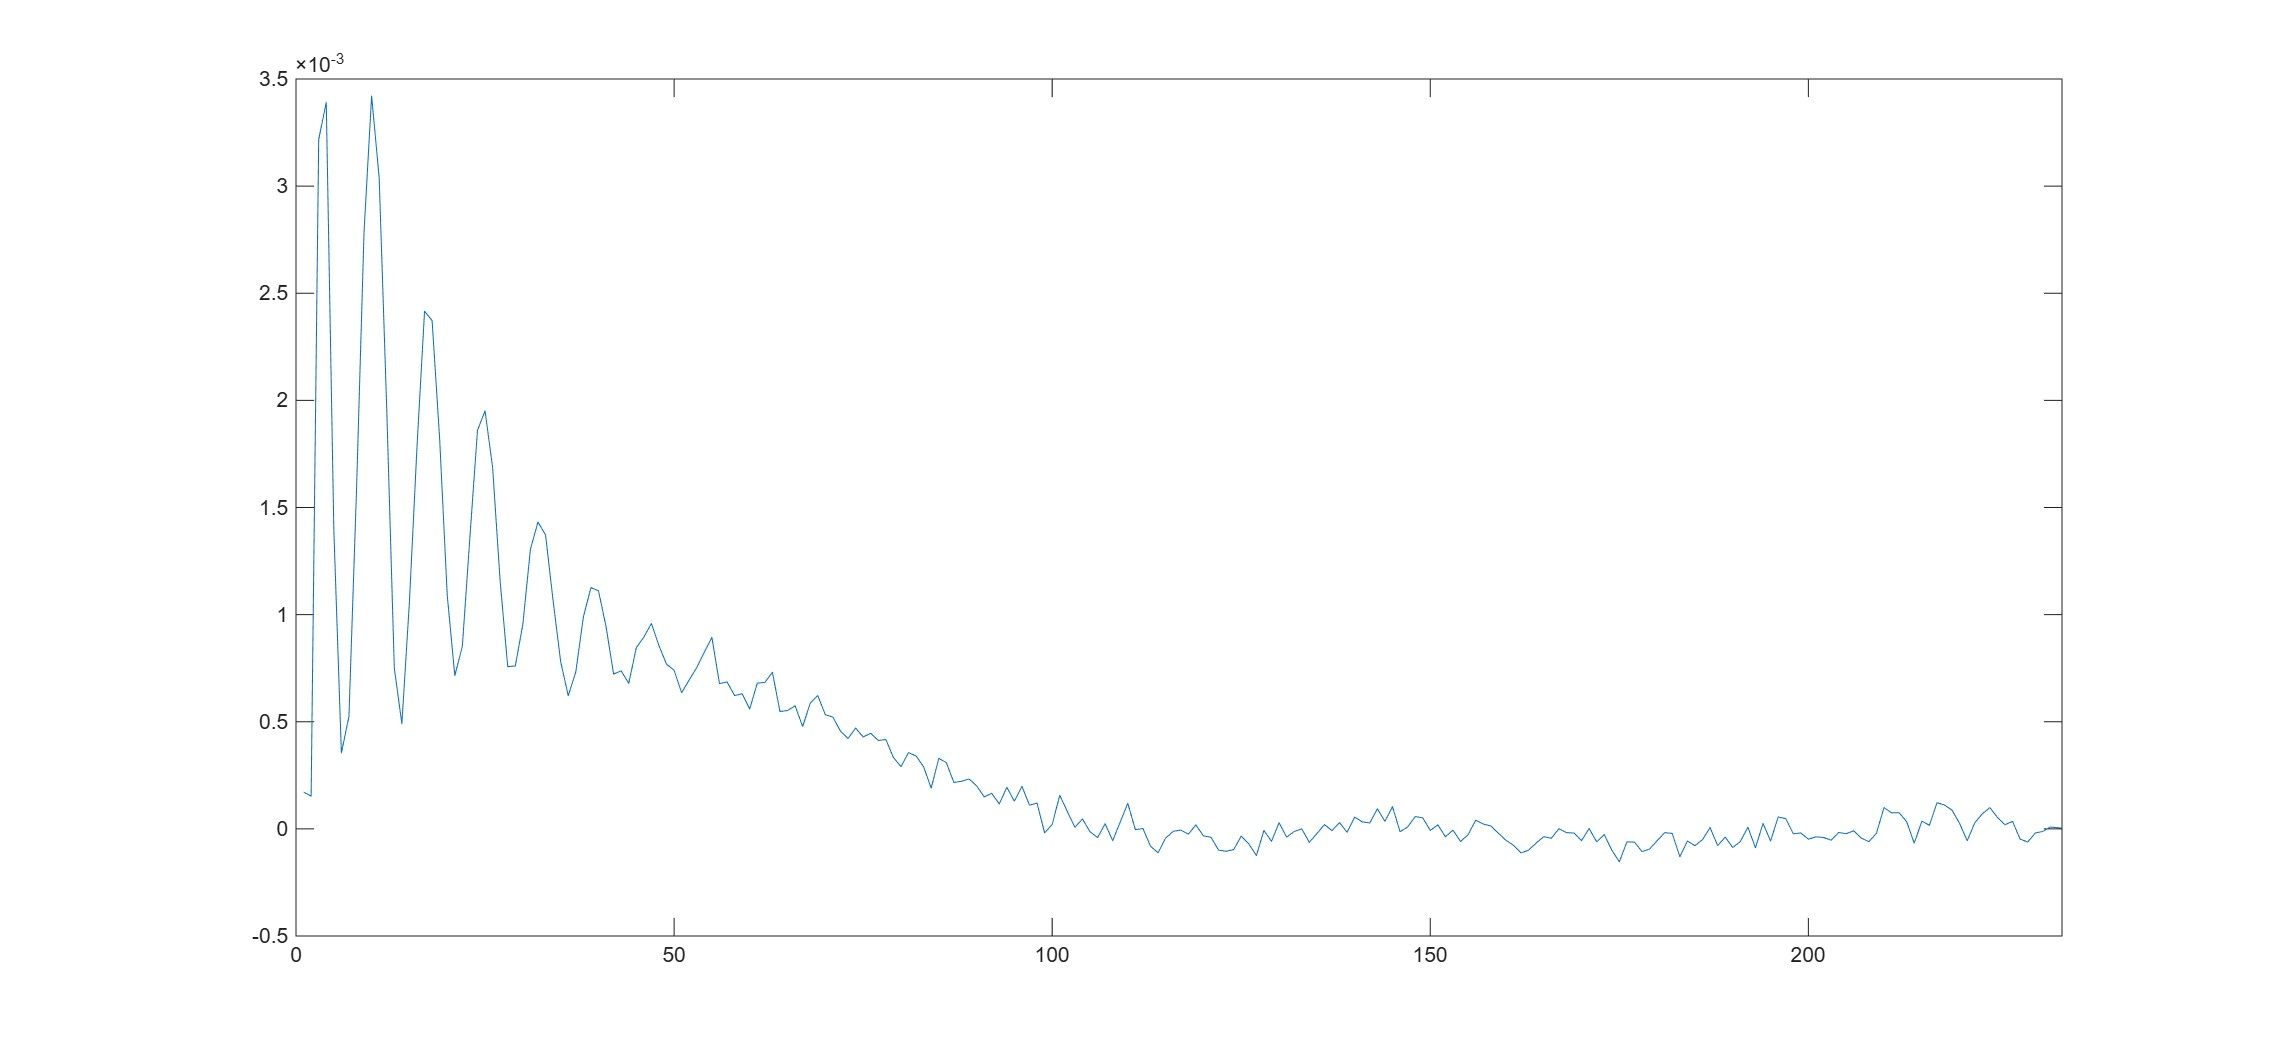
\includegraphics[width=0.8\textwidth]
    {图片/脉冲响应序列.jpg}
    \caption{脉冲响应序列（截取部分）}
    \label{fig:脉冲响应序列}
\end{figure}

\subsection{系统阶次的确定}

得到脉冲响应序列后，可以按照\ref{eq:汉克尔矩阵}的定义构造系统的汉克尔矩阵。根据离散系统分析的相关知识，若系统本身是n阶的，
那么汉克尔矩阵奇异值分解后会有n个主导奇异值。若系统本身是m阶的，那么理想情况下只要构造的汉克尔矩阵阶次n>m即可包含全部的模态。
但是由于采样噪声存在，便是得到的脉冲响应序列并不理想，因此如何选取汉克尔矩阵的阶次
会极大的影响后续的辨识结果。

以永磁同步电机的辨识为例，其求解得到的脉冲响应序列如\ref{fig:脉冲响应序列}所示。可以发现，即使经过了相关运算降噪，
在系统响应结束后仍会有噪声产生的波动，此时系统本身信息接近零，信噪比极低，因此最好的方法是\textbf{选取暂态响应过程构成汉克尔矩阵}。
而构造一个n阶的汉克尔矩阵，需要用到\(g_1\)到\(g_{2n-1}\)的信息。据图求出暂态响应基本结束的时刻（\ref{fig:脉冲响应序列}为20），将其
除以2，即所构造的汉克尔矩阵阶次。在这里选取构造8阶的汉克尔矩阵。

确定汉克尔矩阵阶次后，按照\ref{eq:奇异值分解}进行奇异值分解。在系统阶次判断时，无需关心奇异值的绝对值，只关心奇异值的相对关系，
关心有几个主导（非零）奇异值，因此对齐进行归一化，得到归一化奇异值分解如下图所示。

\begin{figure}[H]
    \centering
    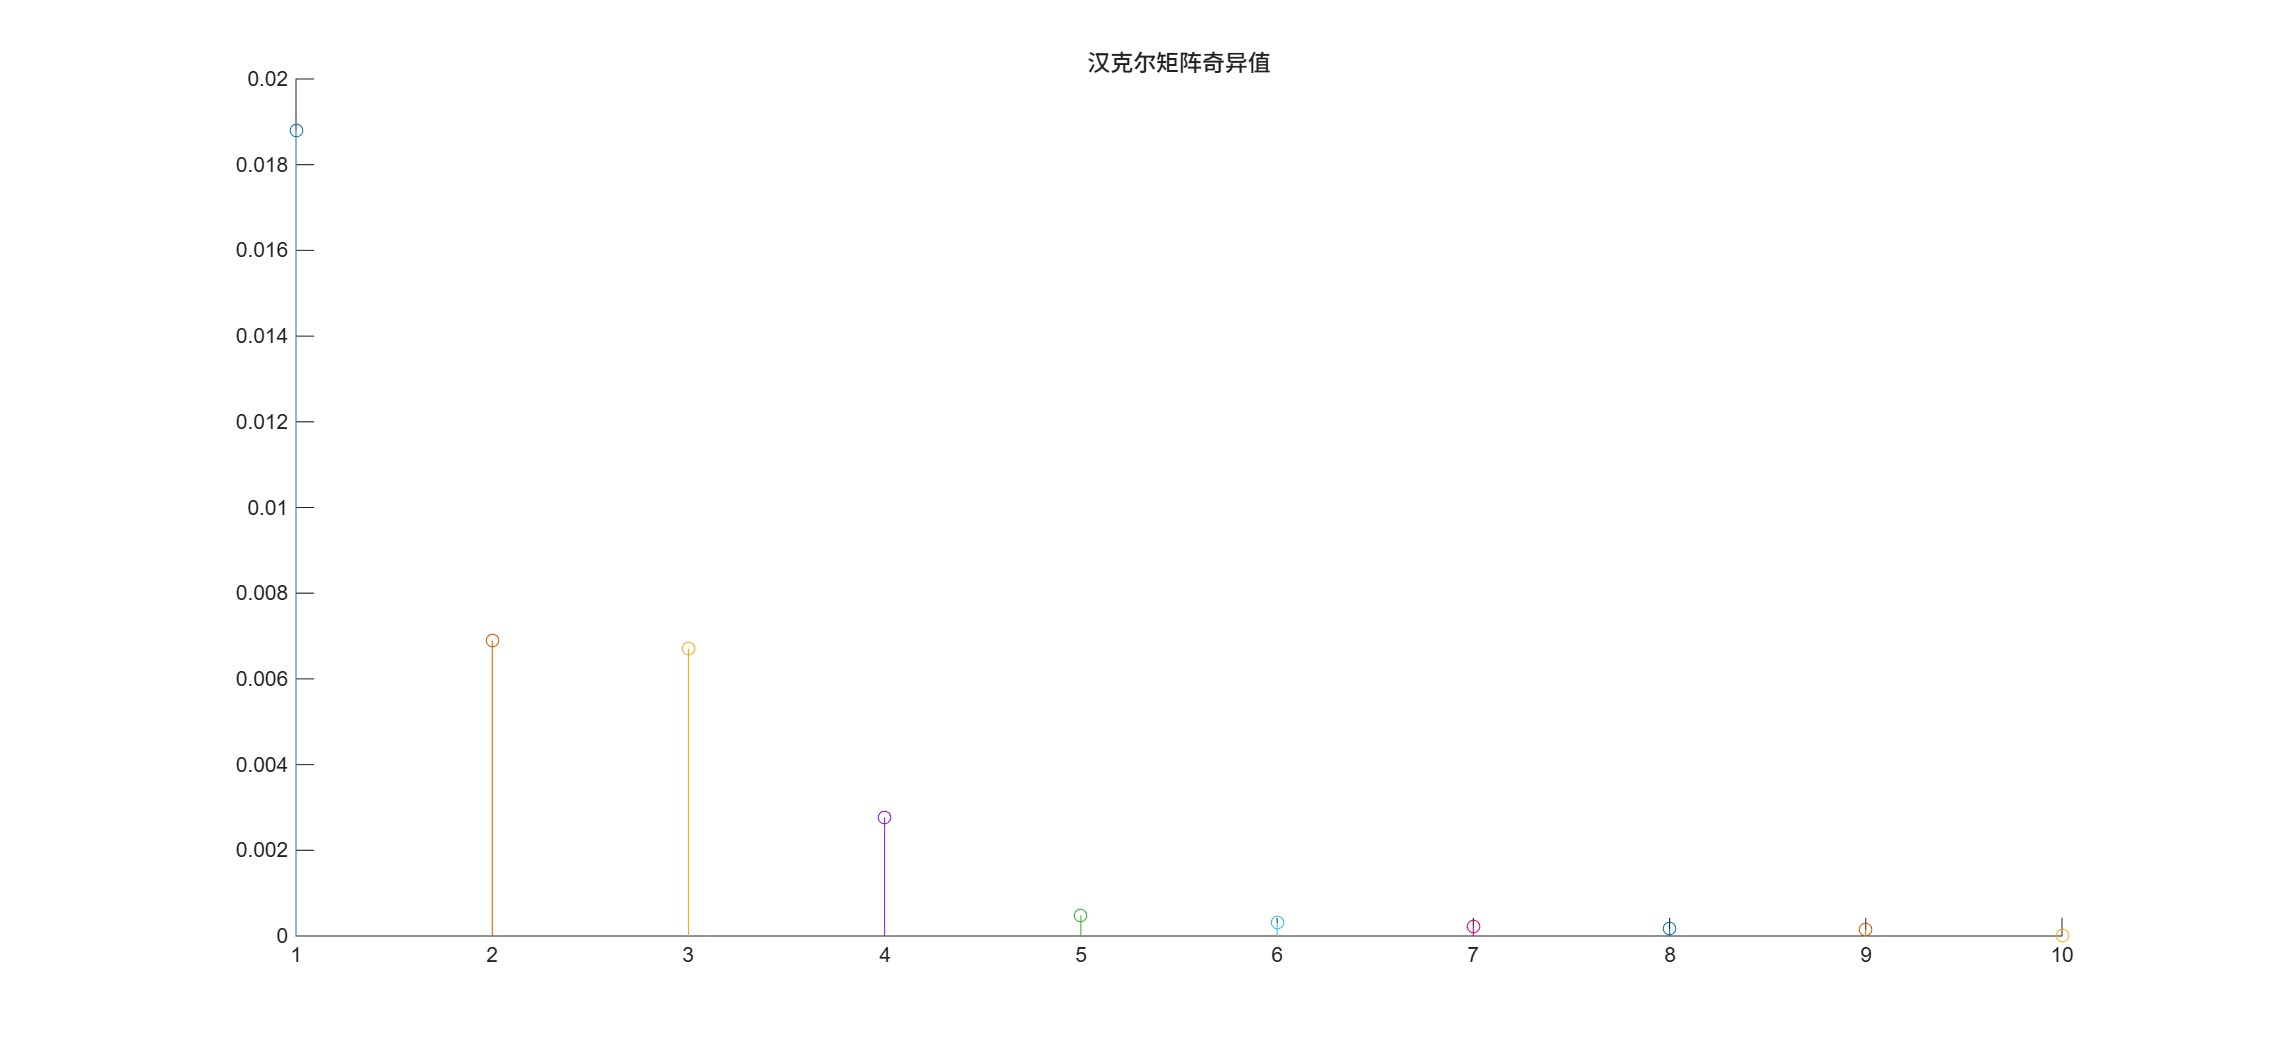
\includegraphics[width=0.8\textwidth]
    {图片/归一化奇异值分解图.jpg}
    \caption{归一化奇异值分解图}
    \label{fig:归一化奇异值分解}
\end{figure}

据图可知，前四个奇异值非零，后续的奇异值基本归零，因此可以判断系统为四阶系统。

\subsection{最小空间实现与传递函数计算}

至此已经得到了系统的汉克尔矩阵\(\mathcal{H}\)，
并完成了奇异值分解得到\(\mathcal{H}=U\Sigma V^T\)，也知道了系统的阶次。如何求解
最小状态空间实现需要的A，B，C，D是接下来讨论的内容。

汉克尔矩阵的定义式为：

\begin{equation*}
    \mathcal{H}=
    \begin{bmatrix}
        g_1 & g_2 & \cdots & g_{n} \\
        g_2 & g_3 & \cdots & g_{n+1} \\
        \vdots & \vdots & \ddots & \vdots \\
        g_{n} & g_{n+1} & \cdots & g_{2n-1}
    \end{bmatrix}
\end{equation*}

根据马尔科夫系数\ref{eq:脉冲响应序列}，可以将汉克尔矩阵改写为：

\begin{equation*}
    \mathcal{H}
    =
    \begin{bmatrix}
        CB & CAB & \cdots & CA^{n-1}B \\
        CAB & CA^2B & \cdots & CA^nB \\
        \vdots & \vdots & \ddots & \vdots \\
        CA^{n-1}B & CA^nB & \cdots & CA^{2n-2}B
    \end{bmatrix}
    =
    \begin{bmatrix}
        C\\CA\\CA^2\\\vdots\\CA^{n-1}
    \end{bmatrix}
    \begin{bmatrix}
        B&AB&A^2B&\cdots&A^{n-1}B
    \end{bmatrix}
     =\mathcal{O}\mathcal{C}
\end{equation*}

也即汉克尔矩阵是能控性矩阵\(\mathcal{C}\)与能观性矩阵\(\mathcal{O}\)之积，
结合汉克尔矩阵的奇异值分解\(\mathcal{H}=U\Sigma V^T\)，系统辨识可以认为：

\begin{equation*}
    \begin{cases}
        \mathcal{O}&=U\Sigma^{0.5} \\
        \mathcal{C}&=\Sigma^{0.5}V^T
    \end{cases}
\end{equation*}

其中\(\Sigma^{0.5}\)表示对奇异值逐个元素取平方根。

求取得到能控性矩阵和能观性矩阵后，根据其定义和确定的系统阶次k，可以得到
\textbf{输入矩阵B由能控性矩阵\(\mathcal{C}\)的第一列前k个元素构成，
输出矩阵为C由能观性矩阵\(\mathcal{O}\)第一行的前k个元素构成}。

为了计算A，可以构造移位汉克尔矩阵：

\begin{equation*}
    \mathcal{H'}=
    \begin{bmatrix}
        g_2 & g_3 & \cdots & g_{n+1} \\
        g_3 & g_4 & \cdots & g_{n+2} \\
        \vdots & \vdots & \ddots & \vdots \\
        g_{n+1} & g_{n+2} & \cdots & g_{2n}
    \end{bmatrix}
\end{equation*}

同样用马尔科夫系数带入得到：

\begin{equation*}
    \mathcal{H'}
    =
    \begin{bmatrix}
        CAB & CA^2B & \cdots & CA^{n}B \\
        CA^2B & CA^3B & \cdots & CA^{n+1}B \\
        \vdots & \vdots & \ddots & \vdots \\
        CA^{n}B & CA^{n+1}B & \cdots & CA^{2n-1}B
    \end{bmatrix}
    =
    \begin{bmatrix}
        C\\CA\\CA^2\\\vdots\\CA^{n-1}
    \end{bmatrix}
    A
    \begin{bmatrix}
        B&AB&A^2B&\cdots&A^{n-1}B
    \end{bmatrix}
    =\mathcal{O}A\mathcal{C}
\end{equation*}

因此A'可以计算为：

\begin{equation*}
    A'=\mathcal{O}^{-1}\mathcal{H'}\mathcal{C}^{-1}
\end{equation*}

而进行截断后，k阶系统实际的\textbf{状态矩阵A由A'的前k行k列的元素构成}。

馈通矩阵D一般由两种做法，第一种是直接忽略视为0，因为实际系统基本不存在随输入信号立刻改变的分量。第二种是辨识认为
\(D=g_0\)。一般为了让辨识结果更符合实际，会选择第二种做法。

得到了四个矩阵后，可以计算得到传递函数\(G(z)=C(zI-A)^{-1}B+D\)，至此，基于Ho-Kalman算法的系统辨识就完成了。